\chapter{User Service}
\section{Abstract}
The user micro-service is the basic component of your micro-service system. It is responsible for all user data and persisting it within a repository. Any other business service that needs user data must contact the user micro-service. The initial user model in the monolith application, receives data from a BAM user controller and stores it in the BAM user repository. In this application, we have gotten rid of the BAM user controller and the services.

\section{Service Architecture}

\begin{figure}[htp]
\centering
\includegraphics[width=18cm]{images/user-package}
\includegraphics[width=18cm]{images/user-class}
\caption{User Service Infrastructure}
\label{fig:lion}
\end{figure}


\begin{figure}[htp]
\centering
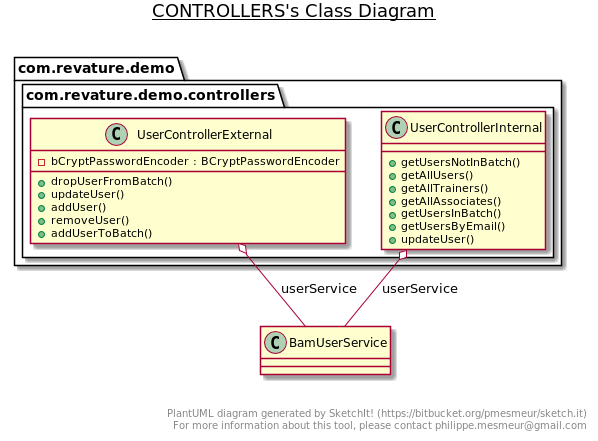
\includegraphics[width=5cm]{images/Usercontrollers}
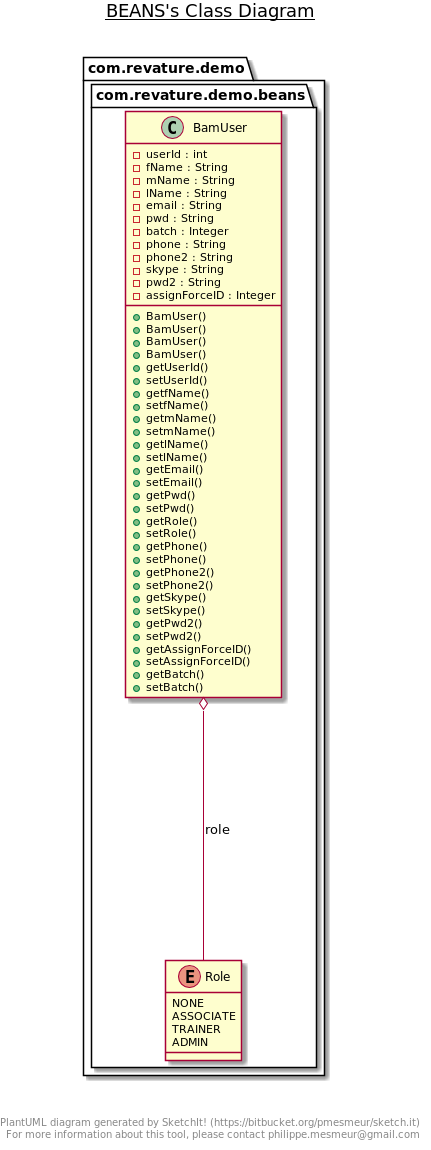
\includegraphics[width=5cm]{images/Userbeans}
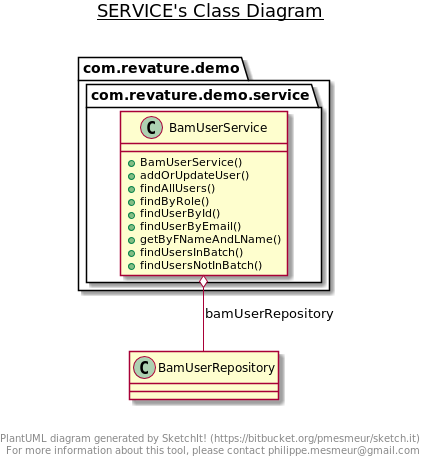
\includegraphics[width=5cm]{images/Userservice}
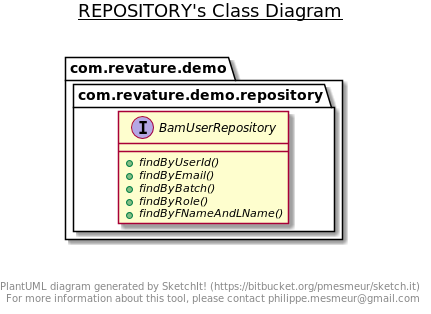
\includegraphics[width=5cm]{images/Userrepository}
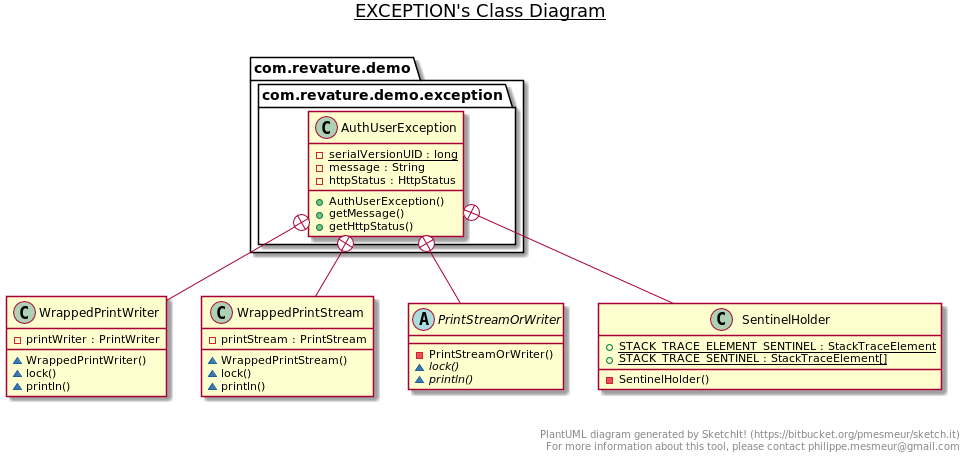
\includegraphics[width=5cm]{images/Userexception}
\caption{User Service Hierarchy}
\label{fig:lion}
\end{figure}